\chapter{Company description}
\section{Organizational chart}\label{org-chart}
Through previous endeavors, research and talks with various people who work in different management positions, we've come to this organizational chart. The diagram \ref{fig:organisational-chart} depicts all required departments and their teams, as well as management positions. Divisions are marked with the same color. The color's saturation denotes the hierarchical position within said department.

\begin{figure}[!ht]
  \centering
  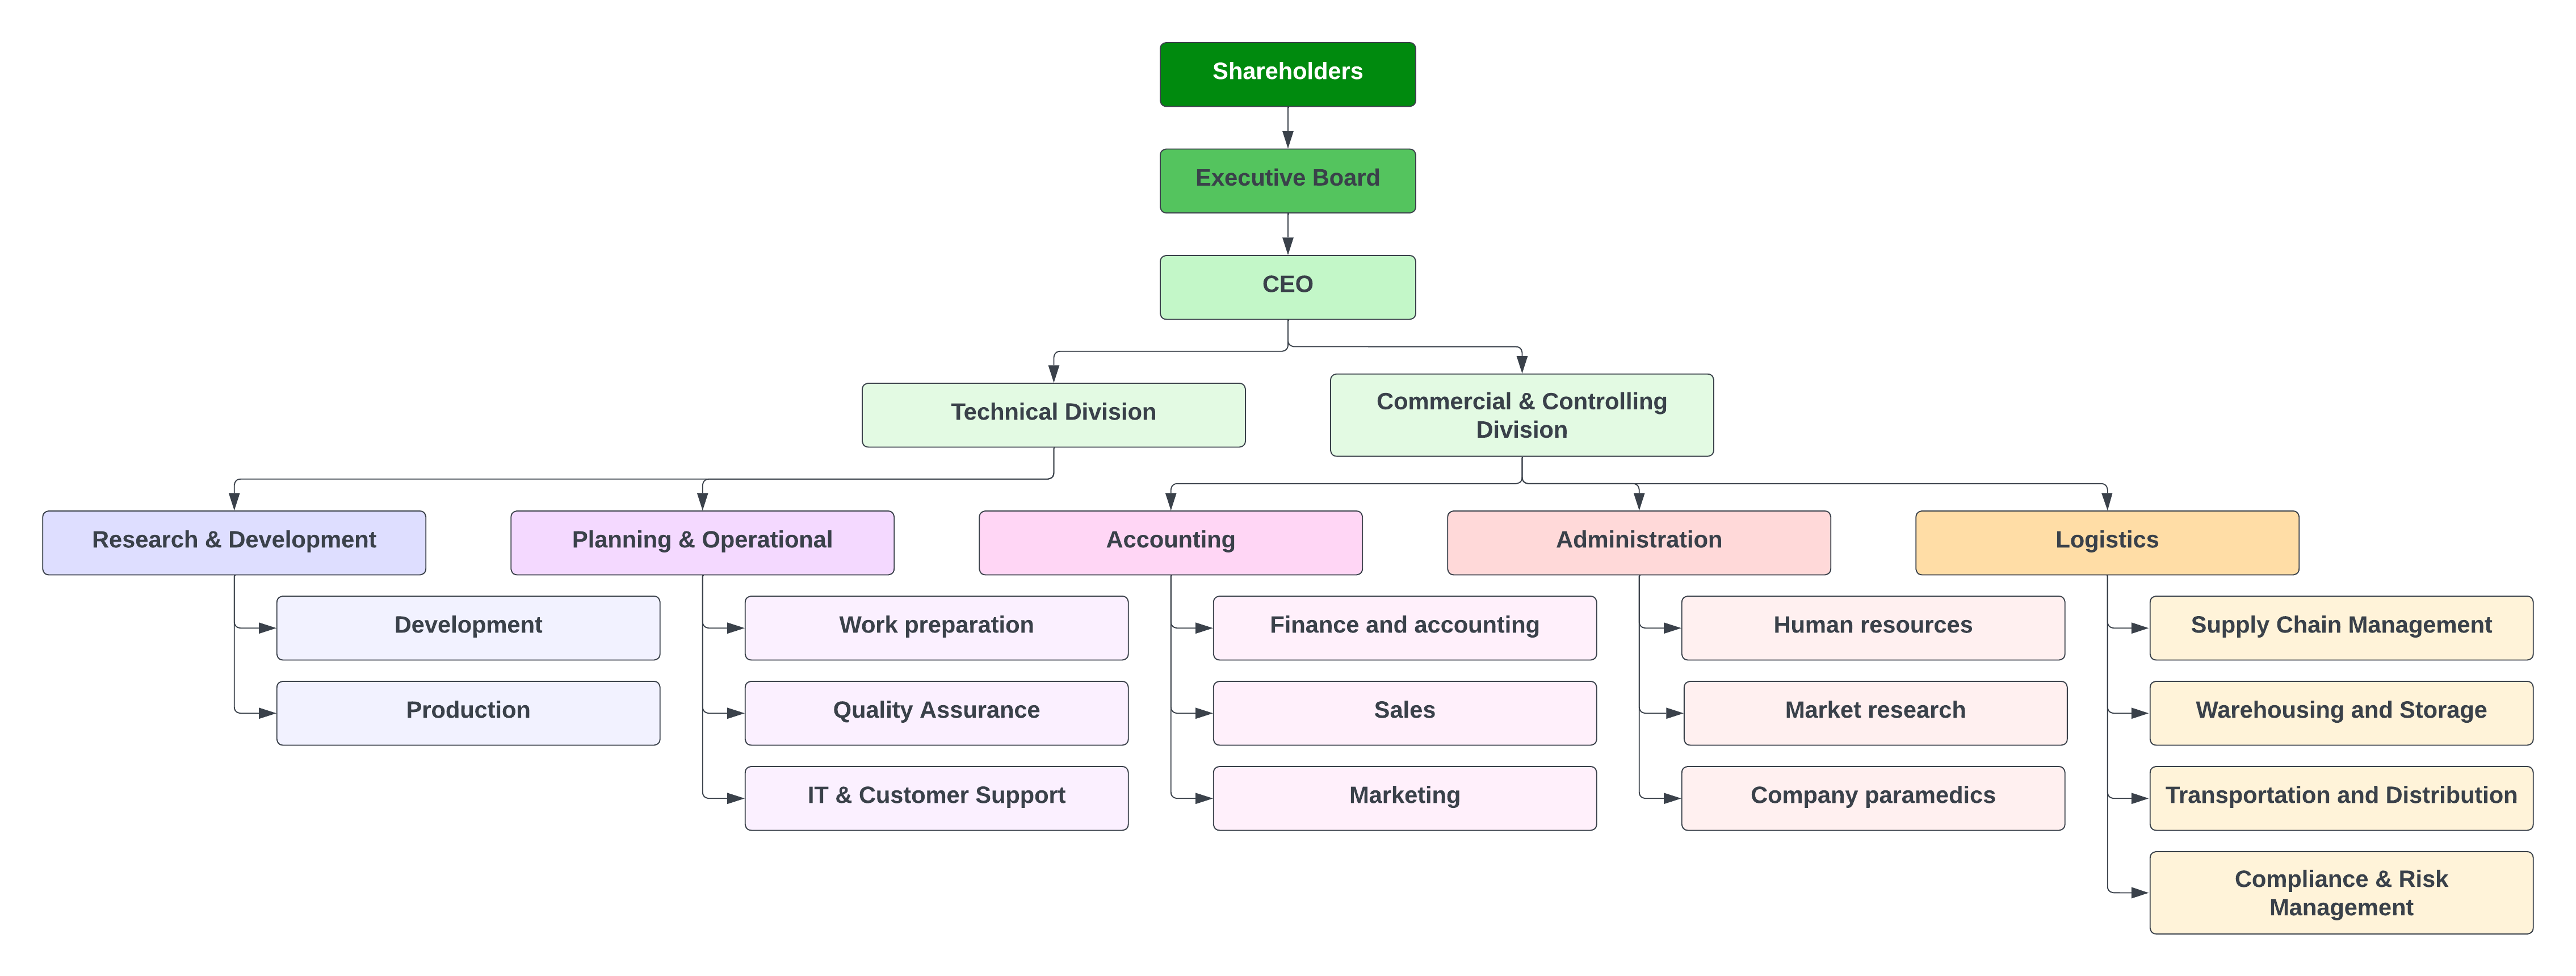
\includegraphics[width=\linewidth]{./images/organisational-chart.png}
  \caption[Organizational chart made with lucidchart.com]{Diagram of the organization}
  \label{fig:organisational-chart}
\end{figure}

This diagram might be more detailed or complex when compared to ones from different startups, but this is by design. It is important that our service works reliably and follows industry standards. To achieve that, we structurally trade a bit of agility for reliability and structure.

Not displayed are ways or means of communication between teams and/or departments. Also, in the future, there might be an additional team whose job it is to ignore department barriers and work on different tasks or enable better communication or a better work flow, depending on the workload of a department.

The following chapters, \ref{org-management} through \ref{org-logistics} will now go into further detail on what each department entails and of what teams it is made of.
\subsection{Management}\label{org-management}
The management division is marked with the color green. This diagram also includes the shareholders and the executive board. This was done in order to paint a complete picture of the company and who has a say in key decisions.
\newline
Shareholders want to maximize their profit. Keeping them safe and happy is detrimental to the long-term success of the company.
\newline
The executive board's and the \acs{ceo}'s job is to lead the company to success and, thus, growth and profitability. They, especially the \acs{ceo}, have the big picture in mind and guide the departments toward said goals. He or she has a say in both the "Technical Division" and the "Commercial \& Controlling Division".
\newline
\newline
If uncertainties arise, consulting is also an option to get an external perspective.
\subsection{\acl{rnd}}\label{org-rnd}
This department is marked with the color indigo.
\newline
By choice, we've structured this technical department into two teams. Both are concerned with "\acl{rnd}", but one focuses on software while the other focuses on hardware. It's detrimental to us, that both hard- and software are done in-house. Having the software team in-house instead of offshore increases the quality, general understanding, and agility of our software. Also, having hardware in-house enables these teams to work closely together, which further increases the quality of the products (and thus also the services) and may also lead to a better work environment, as employees are enabled to innovate and take ownership of their own work. \cite{wang_2022_employee}
\subsection{\acl{pno}}
The "\acl{pno}" department, marked with violet, is made of a less specialized workforce that focuses on supporting other departments, customers, or general processes.
\subsection{Accounting}
The accounting department is featured in a fuchsia color. It encapsulates a general sales and marketing team. These are separated and under the same department by design. Their work may be different, but they need to cooperate with each other frequently, which would be harder if they were in different departments.
Additionally, the "Finance and accounting" team is also under this department. It handles all monetary things.
\subsection{Administration}
The red administration department features a classical "Human resources" team, as well as internal paramedics and the "Market research" team. The last one is concerned with the development of the overall market we operate in and how we maneuver in it. Its findings are detrimental and reported to the CEO, which in turn influences the roadmap of the \ac{rnd} department.
\subsection{Logistics}\label{org-logistics}
Lastly, the logistics department is marked orange. The decision to produce both soft- and hardware in-house requires a bigger logistical effort than if it were done offshore. One team will overlook the supply chain, so that if a global supply bottleneck occurs, we're going to be the least impacted as possible. They're also tasked with prioritizing suppliers who care about sustainability. Two other teams are concerned with the warehousing of materials, while another looks after the transportation of goods.
\section{Vision}
\begin{quote}
  \say{\emph{Build a world where accessible, sustainable, and fast medical care is the standard.}}
\end{quote}

We want to bring a change to medical care and research. Technological advancements can and must be used in this field to give patients the best care they can receive. No dying patient should have to wait unnecessarily for organ transport. No treatment should be delayed because of a traffic jam. There is no reason for a two-ton vehicle for transportation, if one or several drones can get the same job done.
\newline
\newline
Let's be the change that we need.

\section{Mission}
\begin{quote}
  \say{\emph{Reliably support professionals in providing critical health care through innovative means of transportation.}}
\end{quote}

How we want to achieve our vision is by supporting key figures in the health care industry.
\begin{enumerate}
  \item Improve the transportation processes of companies doing research, which would lead to faster time-to-market of new and improved medicines and treatment plans.
  \item Fast, uncomplicated, and reliable transport of timely goods like organ or blood donations.
  \item Fast, uncomplicated, and reliable transport of lab probes or results
  \item Easily and safely accessible medicines for the elderly, handicapped, etc.
  \item Lessen the load on streets and pollution on the environment
\end{enumerate}

\section{Contributions to Sustainability}
We have three means by which we can contribute to sustainability. Each of the following chapters will tackle one of our strategies.
\subsection{Full control over the drones' life cycle}
As mentioned in chapters \ref{org-chart}, \ref{org-rnd} and \ref{org-logistics}, we have full control over not just the service layer of the drones but also the production and logistics that go with them.
\newline
Having this in-house allows us to improve processes and make them more carbon-efficient. Also, having a dedicated "Supply Chain Management" team allows us to compare suppliers and choose the ones best suited for our mission. Furthermore, the transportation efforts are exponentially less, if everything is done under one roof.
\newline
We also have the advantage, that we are allowed to make investments into sustainability, as costs can be spread out over many deliveries for many businesses.
\newline
Lastly, one of our core values is a good work environment where people are encouraged to grow and express themselves. This leads to happier employees and thus has a positive impact on the local community and society as a whole.
\subsection{Precision of transportation}
Conventional transportation of goods requires big buses loaded with many packages to be profitable. Our service offers the solution of direct and precise deliveries. Thus, we are not dependent on things like traffic, other packages, which lessens the overhead of CO2 production. Routing a delivery vehicle to many drop-off points will be less efficient than direct deliveries. Also, a vehicle would waste gas during traffic jams or slow-moving traffic.
\subsection{Electricity}
Compared to conventional transportation, our drones use electricity to transport goods. This makes them, after production, more environmentally sustainable. Usually, this claim enables companies to use it for publicity while offloading the carbon footprint to an energy company. This way, there might still be coal burned to fuel our drones with electricity.
\newline
We want to go the extra mile and buy all, or at least a majority, of the used power from renewable energy sources.
